\ifdefined\inMainDoc\else
\documentclass[12pt,a4paper]{article}
% ================================================================
%  PRÉAMBULE COMMUN - ANNALES CORRIGÉES
%  Université de Kara - FaST - Licence Fondamentale MPC
%  Design optimisé impression noir et blanc
% ================================================================

% -- ENCODAGE & LANGUE --
\usepackage[utf8]{inputenc}
\usepackage[T1]{fontenc}
\usepackage[french]{babel}
\usepackage{lmodern}
\usepackage{microtype}

% -- MISE EN PAGE --
\usepackage[a4paper, top=2.8cm, bottom=2.5cm, left=2.5cm, right=2.5cm, headheight=14pt]{geometry}
\usepackage{setspace}
\setstretch{1.2}
\usepackage{parskip}
\setlength{\parindent}{1.2em}
\setlength{\parskip}{4pt}

% -- MATHS --
\usepackage{amsmath, amssymb, mathtools, amsthm}
\usepackage{mathrsfs}
\usepackage{dsfont}
\usepackage{bm}
\usepackage{cancel}
\usepackage{textcomp}
% Définition de \oiint (intégrale de surface fermée) sans package supplémentaire
\newcommand{\oiint}{\mathop{\iint\!\!\!\!\!\!\!\bigcirc}\limits}

% -- PHYSIQUE & CHIMIE --
\usepackage{physics}
\usepackage{siunitx}
% Lorsque physics est chargé, siunitx omet \qty. On le restaure ici :
\AtBeginDocument{\RenewCommandCopy\qty\SI}
\sisetup{locale = FR, detect-all, output-decimal-marker={,}}
% Commande de substitution pour les unités posant problème avec pdflatex
% (ohm, degreeCelsius, micro, angstrom, percent utilisent des caractères non-ASCII)
\newcommand{\qtyohm}[1]{\ensuremath{\num{#1}\,\Omega}}
\newcommand{\qtydegc}[1]{\ensuremath{\num{#1}\,{}^\circ\text{C}}}
\newcommand{\qtyangstrom}[1]{\ensuremath{\num{#1}\,\text{\AA}}}
\newcommand{\qtypercent}[1]{\ensuremath{\num{#1}\,\%}}
\newcommand{\qtyum}[1]{\ensuremath{\num{#1}\,\mu\text{m}}}
\usepackage[version=4]{mhchem}

% -- GRAPHISMES --
\usepackage{graphicx}
\usepackage{float}
\usepackage{caption}
\usepackage{subcaption}
\usepackage{wrapfig}
\usepackage{tikz}
\usetikzlibrary{calc, arrows.meta, patterns, shapes.geometric}
\usepackage{pgfplots}
\pgfplotsset{compat=1.18}

% -- TABLEAUX --
\usepackage{booktabs}
\usepackage{array}
\usepackage{tabularx}
\usepackage{multirow}

% -- LISTES --
\usepackage{enumitem}
\setlist[enumerate]{topsep=3pt, itemsep=2pt, parsep=0pt}
\setlist[itemize]{topsep=3pt, itemsep=2pt, parsep=0pt, label={.}}

% -- BOÎTES (noir et blanc) --
\usepackage{mdframed}
\usepackage{tcolorbox}
\tcbuselibrary{skins, breakable, theorems}

% Boîte EXERCICE : encadré avec filet épais, fond blanc
\newmdenv[
  linewidth=1.2pt,
  linecolor=black,
  roundcorner=3pt,
  skipabove=10pt,
  skipbelow=6pt,
  innertopmargin=8pt,
  innerbottommargin=8pt,
  innerleftmargin=10pt,
  innerrightmargin=10pt,
  backgroundcolor=white,
  frametitle={\bfseries\small Exercice},
  frametitlealignment=\raggedright,
  frametitleaboveskip=4pt,
  frametitlebelowskip=4pt,
]{boiteexercice}

% Boîte CORRIGÉ : fond gris très clair + filet fin
\newmdenv[
  linewidth=0.6pt,
  linecolor=black,
  leftline=true,
  rightline=false,
  topline=false,
  bottomline=false,
  linecolor=black,
  innerleftmargin=12pt,
  innerrightmargin=8pt,
  innertopmargin=6pt,
  innerbottommargin=6pt,
  backgroundcolor=gray!8,
  skipabove=4pt,
  skipbelow=8pt,
]{boitecorrige}

% Boîte RÉSUMÉ DE COURS : double encadré
\newmdenv[
  linewidth=0.8pt,
  linecolor=black,
  roundcorner=2pt,
  backgroundcolor=gray!12,
  innertopmargin=10pt,
  innerbottommargin=10pt,
  innerleftmargin=12pt,
  innerrightmargin=12pt,
  skipabove=12pt,
  skipbelow=8pt,
]{boiteresume}

% Boîte ATTENTION/REMARQUE : barre gauche épaisse
\newmdenv[
  leftline=true,
  rightline=false,
  topline=false,
  bottomline=false,
  linewidth=3pt,
  linecolor=black,
  backgroundcolor=gray!5,
  innerleftmargin=12pt,
  innerrightmargin=8pt,
  innertopmargin=5pt,
  innerbottommargin=5pt,
  skipabove=6pt,
  skipbelow=6pt,
]{boiteremarque}

% -- DIFFICULTÉ DES EXERCICES --
\newcommand{\facile}{$\star$}
\newcommand{\moyen}{$\star\!\star$}
\newcommand{\difficile}{$\star\!\star\!\star$}
\newcommand{\niveau}[1]{\hfill\textbf{#1}\hspace{2pt}}

% -- EN-TÊTES ET PIEDS DE PAGE --
\usepackage{fancyhdr}
\pagestyle{fancy}
\fancyhf{}
\renewcommand{\headrulewidth}{0.5pt}
\renewcommand{\footrulewidth}{0.3pt}

% -- HYPERLIENS --
\usepackage[hidelinks]{hyperref}
\hypersetup{
    colorlinks=false,
    pdftitle={Annale Corrigée - Licence MPC - Université de Kara}
}

% -- TITRES --
\usepackage{titlesec}
\titleformat{\section}{\Large\bfseries}{\thesection.}{0.8em}{}[\vspace{2pt}\hrule\vspace{4pt}]
\titleformat{\subsection}{\large\bfseries}{\thesubsection.}{0.7em}{}
\titleformat{\subsubsection}{\normalsize\bfseries}{\thesubsubsection.}{0.6em}{}

% -- THÉORÈMES --
\theoremstyle{definition}
\newtheorem{defn}{Définition}[section]
\newtheorem{prop}{Propriété}[section]
\newtheorem{thm}{Théorème}[section]
\newtheorem{corol}{Corollaire}[section]
\newtheorem{exemple}{Exemple}[section]

% -- COMMANDES MATHÉMATIQUES UTILES --
\newcommand{\vect}[1]{\overrightarrow{#1}}
\newcommand{\R}{\mathbb{R}}
\newcommand{\N}{\mathbb{N}}
\newcommand{\Z}{\mathbb{Z}}
\newcommand{\C}{\mathbb{C}}
\renewcommand{\d}{\mathrm{d}}
\newcommand{\deriv}[2]{\dfrac{\d #1}{\d #2}}
\newcommand{\dpart}[2]{\dfrac{\partial #1}{\partial #2}}
\newcommand{\rot}{\overrightarrow{\mathrm{rot}}\,}
\renewcommand{\div}{\mathrm{div}\,}
\renewcommand{\grad}{\overrightarrow{\mathrm{grad}}\,}
\newcommand{\e}{\mathrm{e}}
\newcommand{\ii}{\mathrm{i}}
\renewcommand{\Tr}{\mathrm{Tr}}

% Numérotation des équations par section
\numberwithin{equation}{section}

% -- RÉSULTATS ENCADRÉS --
\newcommand{\res}[1]{\[\boxed{#1}\]}

% -- REMARQUE INLINE --
\newcommand{\rmq}[1]{\begin{boiteremarque}\textbf{Remarque.} #1\end{boiteremarque}}

% -- MISE EN VALEUR DU RÉSULTAT FINAL --
\newcommand{\reponse}[1]{%
  \begin{center}
    \fbox{\begin{minipage}{0.92\textwidth}\centering #1\end{minipage}}
  \end{center}%
}


\lhead{\small\textit{Mécanique des Milieux Continus - Licence 3}}
\rhead{\small\textit{FaST, Université de Kara}}
\cfoot{\thepage}

\begin{document}
\fi

\begin{center}
  {\LARGE\bfseries MÉCANIQUE DES MILIEUX CONTINUS}\\[0.3cm]
  {\normalsize Licence 3 - Physique}\\[0.1cm]
  \rule{0.7\textwidth}{0.8pt}
\end{center}

\section*{Résumé du cours}

\begin{boiteresume}

\textbf{1. Algèbre tensorielle.} Un tenseur d'ordre 2 $\overline{\overline{T}}$ a des composantes $T_{ij}$ dans une base orthonormée. La règle de changement de base : $T'_{ij} = \alpha_{ip}\alpha_{jq}T_{pq}$ (convention d'Einstein). Symétrie ($T_{ij}=T_{ji}$) et antisymétrie ($T_{ij}=-T_{ji}$) sont des propriétés tensorielles. Tout tenseur se décompose : $\overline{\overline{T}} = \overline{\overline{T}}^S + \overline{\overline{T}}^A$ avec $\overline{\overline{T}}^S = \frac{1}{2}(\overline{\overline{T}}+\overline{\overline{T}}^T)$ et $\overline{\overline{T}}^A = \frac{1}{2}(\overline{\overline{T}}-\overline{\overline{T}}^T)$. Produit doublement contracté : $\overline{\overline{S}}:\overline{\overline{T}} = S_{ij}T_{ji}$.

\textbf{2. Cinématique des milieux continus.} Description lagrangienne : $\vec{x} = \vec{\chi}(\vec{X}, t)$ où $\vec{X}$ est la position initiale. Tenseur gradient de la transformation : $F_{iJ} = \partial x_i/\partial X_J$. Tenseur des dilatations de Cauchy-Green à droite : $\overline{\overline{C}} = \overline{\overline{F}}^T\overline{\overline{F}}$. Tenseur des déformations de Green-Lagrange : $\overline{\overline{E}} = \frac{1}{2}(\overline{\overline{C}}-\overline{\overline{I}})$. Jacobien : $J = \det\overline{\overline{F}} > 0$ (conservation de la masse : $\rho J = \rho_0$).

\textbf{3. Cinématique eulérienne.} Tenseur gradient de vitesse : $\overline{\overline{L}} = \overline{\mathrm{grad}}\,\vec{V}$. Décomposition : $\overline{\overline{L}} = \overline{\overline{D}} + \overline{\overline{\Omega}}$ où $\overline{\overline{D}} = \frac{1}{2}(\overline{\overline{L}}+\overline{\overline{L}}^T)$ est le tenseur des taux de déformation et $\overline{\overline{\Omega}} = \frac{1}{2}(\overline{\overline{L}}-\overline{\overline{L}}^T)$ le tenseur des taux de rotation. Conservation de la masse : $\frac{\partial \rho}{\partial t} + \mathrm{div}(\rho\vec{V}) = 0$.

\textbf{4. Mouvement rigidifiant.} Un mouvement est rigidifiant si et seulement si $\overline{\overline{E}} = \overline{\overline{0}}$ (ou de manière équivalente $\overline{\overline{D}} = \overline{\overline{0}}$). Le tenseur des dilatations vaut alors $\overline{\overline{C}} = \overline{\overline{I}}$ : aucune déformation, seul une rotation globale du solide.

\textbf{5. Équations du mouvement.} Équation d'équilibre (quasi-statique) : $\mathrm{div}\,\overline{\overline{\sigma}} + \rho\vec{f} = \vec{0}$. Loi de comportement élastique linéaire (isotrope) : $\overline{\overline{\sigma}} = \lambda(\mathrm{tr}\,\overline{\overline{\varepsilon}})\overline{\overline{I}} + 2\mu\overline{\overline{\varepsilon}}$ avec $\overline{\overline{\varepsilon}}$ le tenseur des petites déformations.

\end{boiteresume}

\newpage
\section{Algèbre tensorielle}

\subsection*{Exercice 1 - Propriétés tensorielles de la symétrie \niveau{\facile}}

\begin{boiteexercice}
Soit $\overline{\overline{S}}$ un tenseur d'ordre 2 symétrique ($S_{ij}=S_{ji}$) dans une base orthonormée $B$. Montrer que cette propriété de symétrie est conservée dans toute autre base orthonormée $B'$.
\end{boiteexercice}

\begin{boitecorrige}
Soit $\alpha_{ij}$ la matrice de passage de $B$ à $B'$. Dans la base $B'$, les composantes de $\overline{\overline{S}}$ sont données par la loi de changement de base :
\[
S'_{ij} = \alpha_{ip}\,\alpha_{jq}\,S_{pq}
\]
On veut montrer que $S'_{ij} = S'_{ji}$. Puisque $S_{pq} = S_{qp}$, on peut intervertir les indices muets $p \leftrightarrow q$ :
\[
S'_{ij} = \alpha_{ip}\,\alpha_{jq}\,S_{pq} = \alpha_{ip}\,\alpha_{jq}\,S_{qp} = \alpha_{jq}\,\alpha_{ip}\,S_{qp}
\]
Or, en renommant les indices muets ($p \to q$, $q \to p$) dans l'expression de $S'_{ji}$ :
\[
S'_{ji} = \alpha_{jp}\,\alpha_{iq}\,S_{pq}
\]
En intervertissant $p \leftrightarrow q$ dans $S'_{ij}$ : $S'_{ij} = \alpha_{jp}\,\alpha_{iq}\,S_{pq} = S'_{ji}$. La symétrie est bien une propriété tensorielle.
\end{boitecorrige}

\subsection*{Exercice 2 - Décomposition d'un tenseur \niveau{\facile}}

\begin{boiteexercice}
\begin{enumerate}
  \item Montrer que tout tenseur $\overline{\overline{T}}$ peut se décomposer en une partie symétrique $\overline{\overline{T}}^S$ et une partie antisymétrique $\overline{\overline{T}}^A$.
  \item Montrer que pour $\overline{\overline{S}}$ symétrique et $\overline{\overline{A}}$ antisymétrique, on a $\overline{\overline{S}}:\overline{\overline{A}} = 0$.
  \item En déduire que $\overline{\overline{S}}:\overline{\overline{T}} = \overline{\overline{S}}:\overline{\overline{T}}^S$.
\end{enumerate}
\end{boiteexercice}

\begin{boitecorrige}
\textbf{1.} On pose :
\[
\overline{\overline{T}}^S = \frac{1}{2}(\overline{\overline{T}}+\overline{\overline{T}}^T), \qquad \overline{\overline{T}}^A = \frac{1}{2}(\overline{\overline{T}}-\overline{\overline{T}}^T)
\]
En composantes : $T^S_{ij} = \frac{1}{2}(T_{ij}+T_{ji}) = T^S_{ji}$ (symétrique) et $T^A_{ij} = \frac{1}{2}(T_{ij}-T_{ji}) = -T^A_{ji}$ (antisymétrique). On vérifie $\overline{\overline{T}}^S + \overline{\overline{T}}^A = \overline{\overline{T}}$.

\textbf{2.} En développant explicitement $\overline{\overline{S}}:\overline{\overline{A}} = S_{ij}A_{ji}$ :
\[
\overline{\overline{S}}:\overline{\overline{A}} = \sum_{i,j} S_{ij}A_{ji}
\]
Les termes diagonaux sont nuls ($A_{ii}=0$ car antisymétrique). Pour les termes hors diagonale, par symétrie $S_{ij}=S_{ji}$ et antisymétrie $A_{ij}=-A_{ji}$ :
\[
S_{12}A_{21} + S_{21}A_{12} = S_{12}A_{21} + S_{12}(-A_{21}) = 0
\]
et de même pour les autres paires. Donc $\overline{\overline{S}}:\overline{\overline{A}} = 0$.

\textbf{3.} Par distributivité et le résultat précédent :
\[
\overline{\overline{S}}:\overline{\overline{T}} = \overline{\overline{S}}:(\overline{\overline{T}}^S + \overline{\overline{T}}^A) = \overline{\overline{S}}:\overline{\overline{T}}^S + \underbrace{\overline{\overline{S}}:\overline{\overline{T}}^A}_{=0} = \overline{\overline{S}}:\overline{\overline{T}}^S
\]
\end{boitecorrige}

\section{Cinématique des milieux continus}

\subsection*{Exercice 3 - Rotation solide \niveau{\moyen}}

\begin{boiteexercice}
On considère le mouvement défini en représentation lagrangienne par ($\omega$ constante positive) :
\[
\begin{cases}
x_1 = X_1\cos(\omega t) - X_2\sin(\omega t)\\
x_2 = X_1\sin(\omega t) + X_2\cos(\omega t)\\
x_3 = X_3
\end{cases}
\]
\begin{enumerate}
  \item Calculer le tenseur gradient $\overline{\overline{F}}$, le tenseur des dilatations $\overline{\overline{C}}$ et le tenseur des déformations $\overline{\overline{E}}$.
  \item À quelle classe particulière ce mouvement appartient-il ? Justifier.
  \item Calculer le jacobien $J$ et en déduire la masse volumique à l'instant $t$.
  \item Calculer les champs de vitesse et d'accélération lagrangiens.
  \item Exprimer $\vec{V}$ et $\vec{\gamma}$ en coordonnées eulériennes. Calculer $\overline{\overline{D}}$ et $\overline{\overline{\Omega}}$.
\end{enumerate}
\end{boiteexercice}

\begin{boitecorrige}
\textbf{1.} Le terme général de $\overline{\overline{F}}$ est $F_{iJ} = \partial x_i/\partial X_J$ :
\[
\overline{\overline{F}} = \begin{pmatrix}\cos\omega t & -\sin\omega t & 0\\ \sin\omega t & \cos\omega t & 0\\ 0 & 0 & 1\end{pmatrix}
\]
Tenseur des dilatations $\overline{\overline{C}} = \overline{\overline{F}}^T\overline{\overline{F}}$ :
\[
\overline{\overline{C}} = \begin{pmatrix}\cos\omega t & \sin\omega t & 0\\ -\sin\omega t & \cos\omega t & 0\\ 0 & 0 & 1\end{pmatrix}\begin{pmatrix}\cos\omega t & -\sin\omega t & 0\\ \sin\omega t & \cos\omega t & 0\\ 0 & 0 & 1\end{pmatrix} = \begin{pmatrix}1&0&0\\0&1&0\\0&0&1\end{pmatrix} = \overline{\overline{I}}
\]
Donc $\overline{\overline{E}} = \frac{1}{2}(\overline{\overline{C}}-\overline{\overline{I}}) = \overline{\overline{0}}$.

\textbf{2.} Puisque $\overline{\overline{E}} = \overline{\overline{0}}$, ce mouvement est \textbf{rigidifiant} : c'est une rotation pure autour de l'axe $\vec{e}_3$ à vitesse angulaire $\omega$.

\textbf{3.} $J = \det\overline{\overline{F}} = \cos^2\omega t + \sin^2\omega t = 1$. La conservation de la masse $\rho J = \rho_0$ donne $\rho = \rho_0$ : la masse volumique est constante.

\textbf{4.} Le champ de vitesse lagrangien $\vec{V} = D\vec{x}/Dt$ :
\[
\begin{cases}
V_1 = -\omega X_1\sin\omega t - \omega X_2\cos\omega t\\
V_2 = \omega X_1\cos\omega t - \omega X_2\sin\omega t\\
V_3 = 0
\end{cases}
\]
L'accélération $\vec{\gamma} = D\vec{V}/Dt$ :
\[
\begin{cases}
\gamma_1 = -\omega^2(X_1\cos\omega t - X_2\sin\omega t) = -\omega^2 x_1\\
\gamma_2 = -\omega^2(X_1\sin\omega t + X_2\cos\omega t) = -\omega^2 x_2\\
\gamma_3 = 0
\end{cases}
\]

\textbf{5.} En inversant la transformation ($X_1 = x_1\cos\omega t + x_2\sin\omega t$, $X_2 = -x_1\sin\omega t + x_2\cos\omega t$), on exprime $\vec{V}$ en coordonnées eulériennes :
\[
\vec{V}(\vec{x},t) = \omega(-x_2\vec{e}_1 + x_1\vec{e}_2)
\]
Le tenseur gradient de vitesse $\overline{\overline{L}} = \overline{\mathrm{grad}}\,\vec{V}$ a pour composantes $L_{ij} = \partial V_i/\partial x_j$ :
\[
\overline{\overline{L}} = \omega\begin{pmatrix}0&-1&0\\1&0&0\\0&0&0\end{pmatrix}
\]
$\overline{\overline{L}}$ est antisymétrique, donc $\overline{\overline{D}} = \overline{\overline{0}}$ et $\overline{\overline{\Omega}} = \overline{\overline{L}}$. Le taux de rotation est $\omega$ autour de $\vec{e}_3$.
\end{boitecorrige}

\subsection*{Exercice 4 - Cinématique d'un tourbillon \niveau{\moyen}}

\begin{boiteexercice}
On considère un mouvement eulérien défini par :
\[
\vec{V}(x_1,x_2) = A(x_1,x_2)\begin{pmatrix}-x_2\\x_1\\0\end{pmatrix}, \quad A = \frac{\alpha}{2\pi(x_1^2+x_2^2)}
\]
où $\alpha$ est une constante positive, défini pour $x_1^2+x_2^2 > 0$.
\begin{enumerate}
  \item De quel type de mouvement s'agit-il qualitativement ?
  \item Calculer la matrice du tenseur gradient de vitesse $\overline{\overline{L}}$.
  \item En déduire $\overline{\overline{D}}$ et $\overline{\overline{\Omega}}$. Commenter.
  \item Calculer $\mathrm{div}\,\vec{V}$ et en déduire la masse volumique à tout instant.
\end{enumerate}
\end{boiteexercice}

\begin{boitecorrige}
\textbf{1.} Les lignes de courant sont des cercles centrés à l'origine. Il s'agit d'un \textbf{tourbillon} (ou vortex) à circulation constante.

\textbf{2.} Avec $A = \alpha/[2\pi(x_1^2+x_2^2)]$, les dérivées partielles de $V_1 = -Ax_2$ et $V_2 = Ax_1$ donnent :
\[
\overline{\overline{L}} = \frac{A}{x_1^2+x_2^2}\begin{pmatrix}2x_1x_2 & x_2^2-x_1^2 & 0\\ x_2^2-x_1^2 & -2x_1x_2 & 0\\ 0 & 0 & 0\end{pmatrix}
\]

\textbf{3.} La partie symétrique $\overline{\overline{D}} = \frac{1}{2}(\overline{\overline{L}}+\overline{\overline{L}}^T)$ et la partie antisymétrique $\overline{\overline{\Omega}} = \frac{1}{2}(\overline{\overline{L}}-\overline{\overline{L}}^T)$ :

On vérifie que $\overline{\overline{L}}$ est \textbf{symétrique} (puisque $L_{12}=L_{21}$ et $L_{11}+L_{22}=0$). Donc $\overline{\overline{D}} = \overline{\overline{L}}$ et $\overline{\overline{\Omega}} = \overline{\overline{0}}$. Le mouvement a des taux de déformation non nuls mais aucune rotation instantanée : paradoxalement, ce tourbillon est \textit{irrotationnel}.

\textbf{4.} $\mathrm{div}\,\vec{V} = \partial V_1/\partial x_1 + \partial V_2/\partial x_2 = \frac{2Ax_1x_2}{x_1^2+x_2^2} + \frac{-2Ax_1x_2}{x_1^2+x_2^2} = 0$.

L'écoulement est incompressible : $\frac{D\rho}{Dt} = -\rho\,\mathrm{div}\,\vec{V} = 0$, donc $\rho = \rho_0$ (constante en tout point et tout instant).
\end{boitecorrige}

\subsection*{Exercice 5 - Petites déformations \niveau{\difficile}}

\begin{boiteexercice}
Un milieu élastique linéaire isotrope (module de Young $E=\qty{210}{GPa}$, coefficient de Poisson $\nu=0{,}3$) est soumis à un état de contrainte uniaxial : $\sigma_{11} = \sigma_0$, toutes les autres composantes nulles.
\begin{enumerate}
  \item Rappeler la loi de comportement de Hooke généralisée reliant $\overline{\overline{\varepsilon}}$ à $\overline{\overline{\sigma}}$.
  \item Calculer toutes les composantes du tenseur des petites déformations $\varepsilon_{ij}$.
  \item Calculer la dilatation volumique $\theta = \mathrm{tr}\,\overline{\overline{\varepsilon}}$.
  \item Calculer les coefficients de Lamé $\lambda$ et $\mu$ (module de cisaillement) en fonction de $E$ et $\nu$.
\end{enumerate}
\end{boiteexercice}

\begin{boitecorrige}
\textbf{1.} Loi de Hooke généralisée (isotrope) :
\[
\varepsilon_{ij} = \frac{1+\nu}{E}\sigma_{ij} - \frac{\nu}{E}(\mathrm{tr}\,\overline{\overline{\sigma}})\delta_{ij}
\]

\textbf{2.} Ici $\mathrm{tr}\,\overline{\overline{\sigma}} = \sigma_0$. On obtient :
\[
\varepsilon_{11} = \frac{1+\nu}{E}\sigma_0 - \frac{\nu}{E}\sigma_0 = \frac{\sigma_0}{E}
\]
\[
\varepsilon_{22} = \varepsilon_{33} = 0 - \frac{\nu}{E}\sigma_0 = -\frac{\nu\sigma_0}{E}
\]
Toutes les composantes de cisaillement ($i\neq j$) sont nulles.

Application numérique : $\varepsilon_{11} = \sigma_0/210\,\text{GPa}$, $\varepsilon_{22}=\varepsilon_{33}=-0{,}3\sigma_0/210\,\text{GPa}$.

\textbf{3.} Dilatation volumique :
\[
\theta = \varepsilon_{11}+\varepsilon_{22}+\varepsilon_{33} = \frac{\sigma_0}{E} - \frac{2\nu\sigma_0}{E} = \frac{(1-2\nu)\sigma_0}{E} = \frac{0{,}4\,\sigma_0}{210\,\text{GPa}}
\]

\textbf{4.} Les coefficients de Lamé :
\[
\mu = \frac{E}{2(1+\nu)} = \frac{210}{2\times1{,}3} \approx \qty{80.8}{GPa}
\]
\[
\lambda = \frac{E\nu}{(1+\nu)(1-2\nu)} = \frac{210\times0{,}3}{1{,}3\times0{,}4} \approx \qty{121}{GPa}
\]
\end{boitecorrige}


\section{Cinématique avancée}

\subsection*{Exercice 6 - Rotation solide en coordonnées polaires \niveau{\difficile}}

\begin{boiteexercice}
On considère le mouvement défini en représentation lagrangienne par ($\omega$ constante positive) :
\[
\begin{cases}
x_1 = X_1\cos(\omega t) - X_2\sin(\omega t)\\
x_2 = X_1\sin(\omega t) + X_2\cos(\omega t)\\
x_3 = X_3
\end{cases}
\]
\begin{enumerate}
  \item Calculer $\overline{\overline{F}}$, $\overline{\overline{C}}$, $\overline{\overline{E}}$. À quelle classe ce mouvement appartient-il ?
  \item Calculer le jacobien $J$ et en déduire la masse volumique.
  \item Calculer les champs de vitesse et d'accélération lagrangiens, puis eulériens. En déduire $\overline{\overline{D}}$ et $\overline{\overline{\Omega}}$.
  \item En coordonnées polaires lagrangiennes $(R,\Theta)$ et eulériennes $(r,\theta)$, exprimer les fonctions $X_r$ et $X_\theta$ définissant le mouvement.
  \item Exprimer le champ de vitesse en coordonnées polaires dans la base $B' = (\vec{e}_r, \vec{e}_\theta, \vec{e}_3)$.
  \item Calculer l'accélération centripète $\gamma_r$ et tangentielle $\gamma_\theta$.
  \item Définir les trajectoires du mouvement.
\end{enumerate}
\end{boiteexercice}

\begin{boitecorrige}
\textbf{1.} $\overline{\overline{F}} = \begin{pmatrix}\cos\omega t & -\sin\omega t & 0\\ \sin\omega t & \cos\omega t & 0\\ 0 & 0 & 1\end{pmatrix}$, $\overline{\overline{C}} = \overline{\overline{F}}^T\overline{\overline{F}} = \overline{\overline{I}}$, donc $\overline{\overline{E}} = \overline{\overline{0}}$ : \textbf{mouvement rigidifiant} (rotation pure).

\textbf{2.} $J = \det\overline{\overline{F}} = \cos^2\omega t + \sin^2\omega t = 1$, donc $\rho = \rho_0$ (masse volumique constante).

\textbf{3.} Champ de vitesse lagrangien $\vec{V} = D\vec{x}/Dt$ :
\[
V_1 = -\omega X_1\sin\omega t - \omega X_2\cos\omega t, \quad V_2 = \omega X_1\cos\omega t - \omega X_2\sin\omega t, \quad V_3 = 0
\]
Accélération lagrangienne : $\gamma_1 = -\omega^2 x_1$, $\gamma_2 = -\omega^2 x_2$, $\gamma_3 = 0$.

En coordonnées eulériennes (en inversant la transformation) :
\[
\vec{V}(\vec{x},t) = \omega(-x_2\vec{e}_1 + x_1\vec{e}_2), \qquad \vec{\gamma} = -\omega^2(x_1\vec{e}_1 + x_2\vec{e}_2)
\]
Le tenseur $\overline{\overline{L}} = \overline{\mathrm{grad}}\,\vec{V}$ est antisymétrique : $\overline{\overline{D}} = \overline{\overline{0}}$ et $\overline{\overline{\Omega}} = \overline{\overline{L}} = \omega\begin{pmatrix}0&-1&0\\1&0&0\\0&0&0\end{pmatrix}$.

\textbf{4.} En passant aux coordonnées polaires : $r = \sqrt{x_1^2+x_2^2} = R$ et $\theta = \Theta + \omega t$.
\[
\begin{cases} r = R \\ \theta = \Theta + \omega t \end{cases}
\]

\textbf{5.} En remplaçant $x_1 = r\cos\theta$, $x_2 = r\sin\theta$ dans $\vec{V} = \omega(-x_2\vec{e}_1 + x_1\vec{e}_2)$, et en utilisant $\vec{e}_\theta = -\sin\theta\,\vec{e}_1 + \cos\theta\,\vec{e}_2$ :
\[
\vec{V} = \omega r\,\vec{e}_\theta \quad\Longrightarrow\quad V_r = 0,\; V_\theta = \omega r,\; V_3 = 0
\]

\textbf{6.} En polaires, $\vec{\gamma} = -\omega^2 r\,\vec{e}_r$ : accélération purement \textbf{centripète}.
\[
\gamma_r = -\omega^2 r, \qquad \gamma_\theta = 0
\]

\textbf{7.} Les trajectoires sont des \textbf{cercles centrés à l'origine}, de rayon $R$ constant, parcourus à vitesse angulaire $\omega$ (constante).
\end{boitecorrige}

\subsection*{Exercice 7 - Étude d'un tourbillon (examen partiel) \niveau{\difficile}}

\begin{boiteexercice}
On considère un mouvement eulérien défini par :
\[
\begin{cases}
V_1 = -A(x_1,x_2)\,x_2\\
V_2 = A(x_1,x_2)\,x_1\\
V_3 = 0
\end{cases}
\quad\text{avec}\quad A(x_1,x_2) = \frac{\alpha}{2\pi(x_1^2+x_2^2)},\; \alpha > 0
\]
défini pour $x_1^2 + x_2^2 > 0$.
\begin{enumerate}
  \item De quel type de mouvement s'agit-il ?
  \item Montrer que la matrice du tenseur gradient de vitesse $\overline{\overline{L}}$ est :
  \[
  \overline{\overline{L}} = \frac{A}{x_1^2+x_2^2}\begin{bmatrix}2x_1x_2 & x_2^2-x_1^2 & 0\\ x_2^2-x_1^2 & -2x_1x_2 & 0\\ 0 & 0 & 0\end{bmatrix}_B
  \]
  \item En déduire $\overline{\overline{\Omega}}$ et $\overline{\overline{D}}$. Commenter.
  \item Calculer $\mathrm{div}\,\vec{V}$ et en déduire la masse volumique.
\end{enumerate}
\end{boiteexercice}

\begin{boitecorrige}
\textbf{1.} Le mouvement est \textbf{plan, permanent et isochore} (tourbillon irrotationnel).

\textbf{2.} On calcule $\partial A/\partial x_i$ puis les dérivées $L_{ij} = \partial V_i/\partial x_j$ :
\[
\frac{\partial A}{\partial x_1} = -A\frac{2x_1}{x_1^2+x_2^2}, \quad \frac{\partial A}{\partial x_2} = -A\frac{2x_2}{x_1^2+x_2^2}
\]
On obtient :
\begin{align*}
L_{11} = \frac{\partial V_1}{\partial x_1} &= \frac{2Ax_1x_2}{x_1^2+x_2^2}, \quad
L_{12} = \frac{\partial V_1}{\partial x_2} = \frac{A(x_2^2-x_1^2)}{x_1^2+x_2^2}\\
L_{21} = \frac{\partial V_2}{\partial x_1} &= \frac{A(x_2^2-x_1^2)}{x_1^2+x_2^2}, \quad
L_{22} = \frac{\partial V_2}{\partial x_2} = \frac{-2Ax_1x_2}{x_1^2+x_2^2}
\end{align*}
La matrice obtenue est bien celle de l'énoncé.

\textbf{3.} La matrice $\overline{\overline{L}}$ est \textbf{symétrique} ($L_{12} = L_{21}$). Donc $\overline{\overline{\Omega}} = \overline{\overline{0}}$ et $\overline{\overline{D}} = \overline{\overline{L}}$. \textit{Paradoxalement, ce tourbillon est irrotationnel} (pas de rotation instantanée) mais présente des taux de déformation non nuls.

\textbf{4.} $\mathrm{div}\,\vec{V} = L_{11} + L_{22} + L_{33} = \frac{2Ax_1x_2 - 2Ax_1x_2}{x_1^2+x_2^2} + 0 = 0$.

Le mouvement est incompressible, donc $D\rho/Dt = 0$ et $\rho = \rho_0$ en tout point et tout instant.
\end{boitecorrige}


\newpage
\section{Mécanique des milieux continus : contraintes et déformations}

\subsection*{Exercice 8 - Tenseur des contraintes : définition et équilibre \niveau{\moyen}}

\begin{boiteexercice}
Le tenseur des contraintes de Cauchy $\overline{\overline{\sigma}}$ est défini par $\vec{t} = \overline{\overline{\sigma}}\cdot\hat{n}$ où $\vec{t}$ est le vecteur contrainte sur la facette de normale $\hat{n}$.
\begin{enumerate}
  \item Définir les composantes normales ($\sigma_{ii}$) et tangentielles ($\sigma_{ij}$, $i\neq j$) du tenseur.
  \item Montrer par un raisonnement sur un tétraèdre de Cauchy que $\overline{\overline{\sigma}}$ est bien un tenseur du second ordre.
  \item En appliquant le bilan des forces sur un volume élémentaire, établir les équations d'équilibre statique :
  \[
  \frac{\partial\sigma_{ij}}{\partial x_j} + f_i = 0
  \]
  où $f_i$ est la composante $i$ de la force volumique.
  \item Montrer par un bilan du moment cinétique que $\overline{\overline{\sigma}}$ est symétrique : $\sigma_{ij} = \sigma_{ji}$.
\end{enumerate}
\end{boiteexercice}

\begin{boitecorrige}
\textbf{1.} Le tenseur des contraintes $\overline{\overline{\sigma}}$ est la matrice $3\times3$ dont l'élément $\sigma_{ij}$ représente la force par unité de surface dans la direction $\vec{e}_i$ exercée sur la facette de normale $\vec{e}_j$.
\begin{itemize}
  \item Composantes \textbf{normales} ($i=j$) : $\sigma_{11},\sigma_{22},\sigma_{33}$ ; contraintes de traction ($>0$) ou compression ($<0$).
  \item Composantes \textbf{tangentielles} ($i\neq j$) : $\sigma_{12},\sigma_{13},\ldots$ ; contraintes de cisaillement.
\end{itemize}

\textbf{2.} On considère un tétraèdre de Cauchy de faces de normales $\hat{n}$ et $-\vec{e}_1$, $-\vec{e}_2$, $-\vec{e}_3$. Le bilan de forces à l'équilibre (en négligeant les forces volumiques d'ordre 3 devant les forces de surface d'ordre 2) donne :
\[
t_i(\hat{n}) = \sigma_{ij}n_j
\]
ce qui montre que le vecteur contrainte $\vec{t}$ est l'image linéaire de $\hat{n}$ par $\overline{\overline{\sigma}}$ : c'est bien un tenseur.

\textbf{3.} Sur un volume élémentaire $dV$, la force de surface est $\oint_{\partial V}\sigma_{ij}n_j\,\d S$. Par le théorème de la divergence et en appliquant la deuxième loi de Newton (équilibre statique $\rho\vec{a}=\vec{0}$) :
\[
\int_V\left(\frac{\partial\sigma_{ij}}{\partial x_j} + f_i\right)\d V = 0
\]
Pour tout volume $V$, cela implique $\dfrac{\partial\sigma_{ij}}{\partial x_j} + f_i = 0$.

\textbf{4.} Le bilan du moment cinétique sur un volume élémentaire, en ne retenant que les termes dominants (d'ordre surface$^2$), donne $\sigma_{ij}-\sigma_{ji}=0$ pour tout $i,j$ : le tenseur des contraintes est symétrique.
\end{boitecorrige}

\subsection*{Exercice 9 - Tenseur des petites déformations \niveau{\moyen}}

\begin{boiteexercice}
Pour un déplacement $\vec{u}(\vec{x})$ petits (approximation linéaire), le tenseur des petites déformations est :
\[
\varepsilon_{ij} = \frac{1}{2}\left(\frac{\partial u_i}{\partial x_j} + \frac{\partial u_j}{\partial x_i}\right)
\]
\begin{enumerate}
  \item Interpréter physiquement les composantes diagonales $\varepsilon_{ii}$ et les composantes de cisaillement $\varepsilon_{ij}$ ($i\neq j$).
  \item Calculer la déformation volumique $\theta = \varepsilon_{kk} = \text{tr}\,\overline{\overline{\varepsilon}} = \text{div}\,\vec{u}$.
  \item Pour le champ de déplacement $\vec{u} = (ax_1, bx_2, cx_3)$ ($a,b,c$ constants), calculer $\overline{\overline{\varepsilon}}$ et $\theta$.
  \item Pour $\vec{u} = \alpha(-x_2, x_1, 0)$ ($\alpha$ petit), calculer $\overline{\overline{\varepsilon}}$. Quel type de déformation s'agit-il ?
  \item Décomposer un déplacement quelconque en une partie déformation pure et une partie rotation.
\end{enumerate}
\end{boiteexercice}

\begin{boitecorrige}
\textbf{1.}
\begin{itemize}
  \item $\varepsilon_{11} = \partial u_1/\partial x_1$ : allongement relatif dans la direction $\vec{e}_1$.
  \item $\varepsilon_{12} = \frac{1}{2}(\partial u_1/\partial x_2 + \partial u_2/\partial x_1)$ : demi-angle de glissement entre les directions $\vec{e}_1$ et $\vec{e}_2$.
\end{itemize}

\textbf{2.} La déformation volumique :
\[
\theta = \varepsilon_{11}+\varepsilon_{22}+\varepsilon_{33} = \frac{\partial u_1}{\partial x_1}+\frac{\partial u_2}{\partial x_2}+\frac{\partial u_3}{\partial x_3} = \text{div}\,\vec{u}
\]

\textbf{3.} Pour $\vec{u} = (ax_1, bx_2, cx_3)$ :
\[
\overline{\overline{\varepsilon}} = \begin{pmatrix}a&0&0\\0&b&0\\0&0&c\end{pmatrix}, \qquad\theta = a+b+c
\]
Déformation homogène sans cisaillement.

\textbf{4.} Pour $\vec{u} = \alpha(-x_2, x_1, 0)$ :
\[
\frac{\partial u_1}{\partial x_1}=0,\quad\frac{\partial u_1}{\partial x_2}=-\alpha,\quad\frac{\partial u_2}{\partial x_1}=\alpha,\quad\frac{\partial u_2}{\partial x_2}=0
\]
\[
\varepsilon_{12} = \frac{1}{2}(-\alpha+\alpha) = 0
\]
Donc $\overline{\overline{\varepsilon}} = \overline{\overline{0}}$ : c'est une \textbf{rotation pure} de petite amplitude $\alpha$ autour de $\vec{e}_3$. Il n'y a aucune déformation.

\textbf{5.} Le gradient de déplacement se décompose en :
\[
\frac{\partial u_i}{\partial x_j} = \varepsilon_{ij} + \omega_{ij}, \quad\omega_{ij} = \frac{1}{2}\left(\frac{\partial u_i}{\partial x_j}-\frac{\partial u_j}{\partial x_i}\right)
\]
$\overline{\overline{\varepsilon}}$ est symétrique (déformation pure) et $\overline{\overline{\omega}}$ est antisymétrique (rotation infinitésimale).
\end{boitecorrige}

\subsection*{Exercice 10 - Loi de Hooke généralisée et coefficients de Lamé \niveau{\moyen}}

\begin{boiteexercice}
Pour un milieu élastique linéaire isotrope, la loi de Hooke généralisée s'écrit :
\[
\sigma_{ij} = \lambda\varepsilon_{kk}\delta_{ij} + 2\mu\varepsilon_{ij}
\]
où $\lambda$ et $\mu$ sont les coefficients de Lamé.
\begin{enumerate}
  \item En inversant, exprimer $\varepsilon_{ij}$ en fonction de $\sigma_{ij}$, $\lambda$ et $\mu$ (ou en termes du module d'Young $E$ et du coefficient de Poisson $\nu$).
  \item Donner les relations entre ($\lambda$, $\mu$) et ($E$, $\nu$).
  \item Pour l'acier ($E = 210$ GPa, $\nu = 0{,}3$), calculer $\lambda$ et $\mu$.
  \item Pour un état de contrainte hydrostatique $\sigma_{ij} = -p\delta_{ij}$, montrer que $\varepsilon_{kk} = -p/K$ où $K = \lambda + 2\mu/3$ est le module de compressibilité.
  \item Quelle est la signification physique de la condition $\nu = 1/2$ ? Et de $\nu < 0$ ?
\end{enumerate}
\end{boiteexercice}

\begin{boitecorrige}
\textbf{1.} On contracte la loi de Hooke : $\sigma_{kk} = (3\lambda+2\mu)\varepsilon_{kk}$. En substituant dans $\sigma_{ij}$ :
\[
\varepsilon_{ij} = \frac{1}{2\mu}\sigma_{ij} - \frac{\lambda}{2\mu(3\lambda+2\mu)}\sigma_{kk}\delta_{ij}
\]

\textbf{2.} Par identification avec la loi de Hooke en termes de $E$ et $\nu$ :
\[
\mu = \frac{E}{2(1+\nu)}, \qquad \lambda = \frac{E\nu}{(1+\nu)(1-2\nu)}
\]
Réciproquement :
\[
E = \frac{\mu(3\lambda+2\mu)}{\lambda+\mu}, \qquad \nu = \frac{\lambda}{2(\lambda+\mu)}
\]

\textbf{3.} Pour l'acier :
\[
\mu = \frac{210}{2\times1{,}3} \approx 80{,}8\;\text{GPa}, \qquad \lambda = \frac{210\times0{,}3}{1{,}3\times0{,}4} \approx 121{,}2\;\text{GPa}
\]

\textbf{4.} Pour $\sigma_{ij} = -p\delta_{ij}$ : la loi inverse donne $\varepsilon_{ij} = \frac{-p}{3\lambda+2\mu}\delta_{ij}$, soit $\varepsilon_{kk} = \frac{-3p}{3\lambda+2\mu}$. En posant $K = (3\lambda+2\mu)/3 = \lambda+2\mu/3$ :
\[
\varepsilon_{kk} = -\frac{p}{K}
\]

\textbf{5.} $\nu=1/2$ : $\lambda\to\infty$, $K\to\infty$, matériau incompressible (caoutchouc). Pour $\nu<0$ (matériaux auxétiques, rares) : le matériau se dilate transversalement sous traction axiale.
\end{boitecorrige}

\subsection*{Exercice 11 - Ondes élastiques dans un solide \niveau{\difficile}}

\begin{boiteexercice}
Dans un solide élastique isotrope de densité $\rho$, de coefficients de Lamé $\lambda$ et $\mu$, les ondes de déplacement $\vec{u}$ vérifient l'équation :
\[
\rho\ddot{u}_i = (\lambda+\mu)\frac{\partial}{\partial x_i}(\text{div}\,\vec{u}) + \mu\Delta u_i
\]
\begin{enumerate}
  \item En décomposant $\vec{u} = \vec{\nabla}\phi + \vec{\nabla}\wedge\vec{\psi}$ (décomposition de Helmholtz), montrer que $\phi$ et $\vec{\psi}$ vérifient des équations d'onde.
  \item Identifier la vitesse des ondes longitudinales $V_L = \sqrt{(\lambda+2\mu)/\rho}$ et des ondes transversales $V_T = \sqrt{\mu/\rho}$.
  \item Pour l'acier ($\rho = 7800$ kg.m$^{-3}$, $E = 210$ GPa, $\nu = 0{,}3$), calculer $V_L$ et $V_T$.
  \item Montrer que $V_L > V_T$ toujours. En déduire que dans un séisme, l'onde primaire P arrive avant l'onde secondaire S.
  \item Quelle est la nature des déformations pour une onde longitudinale et pour une onde transversale ?
\end{enumerate}
\end{boiteexercice}

\begin{boitecorrige}
\textbf{1.} Avec $\vec{u} = \vec{\nabla}\phi + \vec{\nabla}\wedge\vec{\psi}$, on a $\text{div}\,\vec{u} = \Delta\phi$ et $\vec{\nabla}\wedge\vec{u} = \Delta\vec{\psi}$.

En substituant dans l'équation du mouvement et en séparant les parties scalaire et vectorielle :
\[
\rho\ddot\phi = (\lambda+2\mu)\Delta\phi \quad\text{(potentiel scalaire)}
\]
\[
\rho\ddot{\vec{\psi}} = \mu\Delta\vec{\psi} \quad\text{(potentiel vecteur)}
\]

\textbf{2.} Les vitesses sont donc :
\[
V_L = \sqrt{\frac{\lambda+2\mu}{\rho}} \quad\text{(onde longitudinale, P)}, \qquad V_T = \sqrt{\frac{\mu}{\rho}} \quad\text{(onde transversale, S)}
\]

\textbf{3.} Pour l'acier : $\mu = 80{,}8$ GPa, $\lambda = 121{,}2$ GPa.
\begin{align*}
V_L &= \sqrt{\frac{(121{,}2+2\times80{,}8)\times10^9}{7800}} = \sqrt{\frac{282{,}8\times10^9}{7800}}\approx\sqrt{36{,}3\times10^6}\approx 6020\;\text{m.s}^{-1}\\
V_T &= \sqrt{\frac{80{,}8\times10^9}{7800}}\approx\sqrt{10{,}36\times10^6}\approx 3220\;\text{m.s}^{-1}
\end{align*}

\textbf{4.} Puisque $\lambda+2\mu = \lambda + 2\mu > \mu$ (car $\lambda>0$ et $\mu>0$), on a toujours $V_L > V_T$. Dans un séisme, l'onde P (longitudinale) est plus rapide : elle arrive la première aux sismographes.

\textbf{5.}
\begin{itemize}
  \item Onde longitudinale (P) : $\vec{\nabla}\wedge\vec{u}=\vec{0}$, le déplacement est parallèle à la direction de propagation. C'est une onde de compression/dilatation.
  \item Onde transversale (S) : $\text{div}\,\vec{u}=0$, le déplacement est perpendiculaire à la direction de propagation. C'est une onde de cisaillement.
\end{itemize}
\end{boitecorrige}

\subsection*{Exercice 12 - Torsion d'un cylindre circulaire \niveau{\difficile}}

\begin{boiteexercice}
On considère un cylindre circulaire de rayon $R$ et de longueur $L$, soumis à un moment de torsion $M_t$ appliqué à ses deux extrémités.
\begin{enumerate}
  \item On suppose que le champ de déplacement est $u_r = 0$, $u_\theta = r\alpha z/L$, $u_z = 0$, où $\alpha$ est l'angle de torsion entre les deux extrémités. Calculer les composantes non nulles du tenseur des petites déformations.
  \item Appliquer la loi de Hooke pour calculer les contraintes non nulles.
  \item Vérifier que les équations d'équilibre sont satisfaites.
  \item Calculer le moment de torsion $M_t = \int_0^R\sigma_{\theta z}\cdot r\cdot 2\pi r\,\d r$ et en déduire l'angle $\alpha$ en fonction de $M_t$, $L$, $\mu$ et $R$.
\end{enumerate}
\end{boiteexercice}

\begin{boitecorrige}
\textbf{1.} Les composantes du tenseur des petites déformations en coordonnées cylindriques pour $\vec{u} = u_\theta(r,z)\vec{e}_\theta$ :
\[
\varepsilon_{\theta z} = \frac{1}{2}\left(\frac{\partial u_\theta}{\partial z} + \frac{1}{r}\frac{\partial u_z}{\partial\theta}\right) = \frac{1}{2}\cdot\frac{r\alpha}{L}
\]
Toutes les autres composantes sont nulles. La seule déformation non nulle est le cisaillement $\varepsilon_{\theta z} = r\alpha/(2L)$.

\textbf{2.} Par la loi de Hooke $\sigma_{ij} = 2\mu\varepsilon_{ij}$ (les termes diagonaux sont nuls car $\varepsilon_{kk}=0$) :
\[
\sigma_{\theta z} = 2\mu\varepsilon_{\theta z} = \frac{\mu r\alpha}{L}
\]
La contrainte de cisaillement est proportionnelle à $r$ : elle est nulle sur l'axe et maximale à $r=R$.

\textbf{3.} En l'absence de forces volumiques, les équations d'équilibre sont $\partial\sigma_{ij}/\partial x_j = 0$. Ici $\sigma_{\theta z} = \mu r\alpha/L$ dépend de $r$ mais pas de $z$ ni $\theta$, et l'équation d'équilibre en $z$ donne $\partial\sigma_{\theta z}/\partial\theta + \partial\sigma_{zz}/\partial z = 0$ : satisfait.

\textbf{4.} Moment de torsion :
\[
M_t = \int_0^R\sigma_{\theta z}\cdot r\cdot 2\pi r\,\d r = 2\pi\frac{\mu\alpha}{L}\int_0^R r^3\,\d r = 2\pi\frac{\mu\alpha}{L}\cdot\frac{R^4}{4} = \frac{\pi\mu\alpha R^4}{2L}
\]
En posant $I_p = \pi R^4/2$ (moment polaire d'inertie) :
\[
\alpha = \frac{M_t L}{\mu I_p} = \frac{2M_t L}{\mu\pi R^4}
\]
C'est la formule de Saint-Venant pour la torsion d'un cylindre circulaire.
\end{boitecorrige}

\subsection*{Exercice 13 - Contraintes et déformations en 2D : état plan \niveau{\moyen}}

\begin{boiteexercice}
On considère un état de contrainte plane ($\sigma_{i3}=0$ pour tout $i$) avec :
\[
\sigma_{11} = 100\;\text{MPa},\quad\sigma_{22} = -50\;\text{MPa},\quad\sigma_{12} = 40\;\text{MPa}
\]
\begin{enumerate}
  \item Calculer les contraintes principales $\sigma_1$ et $\sigma_2$ (valeurs propres de $\overline{\overline{\sigma}}$).
  \item Calculer les directions principales.
  \item Calculer la contrainte de cisaillement maximale $\tau_{\max}$ et la contrainte normale sur cette facette.
  \item Le milieu est de l'acier ($E=210$ GPa, $\nu=0{,}3$). Calculer toutes les déformations $\varepsilon_{ij}$.
\end{enumerate}
\end{boiteexercice}

\begin{boitecorrige}
\textbf{1.} Valeurs propres de $\begin{pmatrix}100&40\\40&-50\end{pmatrix}$ :
\[
\sigma_{1,2} = \frac{\sigma_{11}+\sigma_{22}}{2}\pm\sqrt{\left(\frac{\sigma_{11}-\sigma_{22}}{2}\right)^2+\sigma_{12}^2}
\]
\[
= \frac{50}{1}\pm\sqrt{75^2+40^2} = 25\pm\sqrt{5625+1600} = 25\pm\sqrt{7225} = 25\pm85
\]
\[
\sigma_1 = 110\;\text{MPa},\quad\sigma_2 = -60\;\text{MPa}
\]

\textbf{2.} Direction principale associée à $\sigma_1$ : $\tan(2\theta) = \frac{2\sigma_{12}}{\sigma_{11}-\sigma_{22}} = \frac{80}{150}\approx 0{,}533$, donc $2\theta\approx 28°$, soit $\theta\approx 14°$.

\textbf{3.} Cisaillement maximum :
\[
\tau_{\max} = \frac{\sigma_1-\sigma_2}{2} = \frac{110-(-60)}{2} = 85\;\text{MPa}
\]
La contrainte normale sur la facette de cisaillement maximum est $(\sigma_1+\sigma_2)/2 = 25$ MPa.

\textbf{4.} Loi de Hooke inverse :
\begin{align*}
\varepsilon_{11} &= \frac{1}{E}(\sigma_{11}-\nu\sigma_{22}) = \frac{100+0{,}3\times50}{210\times10^3} = \frac{115}{210\times10^3}\approx 548\;\mu\text{m/m}\\
\varepsilon_{22} &= \frac{1}{E}(\sigma_{22}-\nu\sigma_{11}) = \frac{-50-30}{210\times10^3}\approx -381\;\mu\text{m/m}\\
\varepsilon_{12} &= \frac{\sigma_{12}}{2\mu} = \frac{40}{2\times80{,}8\times10^3}\approx 247\;\mu\text{m/m}\\
\varepsilon_{33} &= \frac{-\nu}{E}(\sigma_{11}+\sigma_{22}) = \frac{-0{,}3\times50}{210\times10^3}\approx -71\;\mu\text{m/m}
\end{align*}
\end{boitecorrige}


\subsection*{Exercice 14 - Déformations principales d'un tenseur \niveau{\difficile}}

\begin{boiteexercice}
Soit un milieu soumis à un tenseur de déformation $\overline{\overline{E}}$ dont la matrice dans la base $B=(\vec{e}_1,\vec{e}_2,\vec{e}_3)$ est :
\[
\overline{\overline{E}} = \begin{bmatrix}3&2&4\\2&3&4\\4&4&1\end{bmatrix}_B
\]
\begin{enumerate}
  \item Calculer la trace $E_I = \mathrm{tr}\,\overline{\overline{E}}$, le déterminant $E_{III}$ et la matrice $\overline{\overline{E}}^2$. En déduire le second invariant $E_{II} = \frac{1}{2}\left[(\mathrm{tr}\,\overline{\overline{E}})^2 - \mathrm{tr}(\overline{\overline{E}}^2)\right]$. En déduire sans calcul le polynôme caractéristique.
  \item Développer $\det(\overline{\overline{E}}-\lambda\overline{\overline{I}})$ et retrouver ce polynôme.
  \item Factoriser ce polynôme sous la forme $-(\lambda-E_1)(\lambda-E_2)(\lambda-E_3)$. En déduire les déformations principales et la forme de $\overline{\overline{E}}$ dans sa base principale.
  \item Ordonner les déformations principales. Calculer le vecteur propre $\vec{b}_2$ correspondant à $E_2$.
\end{enumerate}
\end{boiteexercice}

\begin{boitecorrige}
\textbf{1.} Trace :
\[
E_I = \mathrm{tr}\,\overline{\overline{E}} = 3+3+1 = 7
\]
Déterminant (règle de Sarrus) :
\[
E_{III} = \det\overline{\overline{E}} = 3\cdot3\cdot1 + 2\cdot4\cdot4 + 4\cdot2\cdot4 - 4\cdot3\cdot4 - 4\cdot4\cdot3 - 1\cdot2\cdot2 = 9+32+32-48-48-4 = -27
\]
Carré du tenseur :
\[
\overline{\overline{E}}^2 = \begin{bmatrix}3&2&4\\2&3&4\\4&4&1\end{bmatrix}\begin{bmatrix}3&2&4\\2&3&4\\4&4&1\end{bmatrix} = \begin{bmatrix}29&28&24\\28&29&24\\24&24&33\end{bmatrix}
\]
$\mathrm{tr}(\overline{\overline{E}}^2) = 29+29+33 = 91$. Second invariant :
\[
E_{II} = \frac{1}{2}(7^2 - 91) = \frac{1}{2}(49-91) = -21
\]
Polynôme caractéristique :
\[
\det(\overline{\overline{E}}-\lambda\overline{\overline{I}}) = -\lambda^3 + E_I\lambda^2 - E_{II}\lambda + E_{III} = -\lambda^3 + 7\lambda^2 + 21\lambda - 27
\]

\textbf{2.} Calcul direct du déterminant :
\[
\overline{\overline{E}}-\lambda\overline{\overline{I}} = \begin{bmatrix}3-\lambda&2&4\\2&3-\lambda&4\\4&4&1-\lambda\end{bmatrix}
\]
En développant par la règle de Sarrus :
\begin{align*}
\det(\overline{\overline{E}}-\lambda\overline{\overline{I}}) &= (3-\lambda)^2(1-\lambda)+32+32 - 4(3-\lambda)\cdot4 - 4\cdot4(3-\lambda) - (1-\lambda)\cdot4\\
&= -\lambda^3 + 7\lambda^2 + 21\lambda - 27
\end{align*}
On retrouve bien le résultat de la question 1.

\textbf{3.} On cherche à factoriser directement le déterminant. En soustrayant la colonne C2 de la colonne C1 :
\[
\det(\overline{\overline{E}}-\lambda\overline{\overline{I}}) = \begin{vmatrix}1-\lambda&2&4\\\lambda-1&3-\lambda&4\\0&4&1-\lambda\end{vmatrix} = (\lambda-1)\begin{vmatrix}-1&2&4\\1&3-\lambda&4\\0&4&1-\lambda\end{vmatrix}
\]
En ajoutant L1 à L2 puis en développant :
\[
= -(\lambda-1)\begin{vmatrix}5-\lambda&8\\4&1-\lambda\end{vmatrix} = -(\lambda-1)\left[(5-\lambda)(1-\lambda)-32\right]
\]
\[
= -(\lambda-1)(\lambda^2-6\lambda-27) = -(\lambda-1)(\lambda-9)(\lambda+3)
\]
Les déformations principales sont $E_1=9$, $E_2=1$, $E_3=-3$, et dans la base principale :
\[
\overline{\overline{E}} = \begin{bmatrix}9&0&0\\0&1&0\\0&0&-3\end{bmatrix}_{\text{base principale}}
\]

\textbf{4.} Ordonnées : $E_1=9 > E_2=1 > E_3=-3$. Vecteur propre $\vec{b}_2$ associé à $E_2=1$ : $(\overline{\overline{E}}-\overline{\overline{I}})\vec{b}_2=\vec{0}$ donne :
\[
\begin{bmatrix}2&2&4\\2&2&4\\4&4&0\end{bmatrix}\begin{bmatrix}b_{2,1}\\b_{2,2}\\b_{2,3}\end{bmatrix}=\vec{0}
\]
De la troisième équation $4b_{2,1}+4b_{2,2}=0$, on tire $b_{2,1}=-b_{2,2}$. De la première : $2b_{2,1}+2b_{2,2}+4b_{2,3}=0$, soit $b_{2,3}=0$. En normalisant :
\[
\vec{b}_2 = \frac{\sqrt{2}}{2}\vec{e}_1 - \frac{\sqrt{2}}{2}\vec{e}_2
\]
\end{boitecorrige}


\subsection*{Exercice 15 - Tenseur de Cauchy à partir de mesures de forces \niveau{\difficile}}

\begin{boiteexercice}
Soit un milieu continu dont l'état de contrainte est homogène et stationnaire. On considère un domaine matériel en forme de tétraèdre dont les arêtes parallèles aux axes ont une longueur $c$ (voir figure). Un expérimentateur mesure :
\begin{itemize}
  \item La composante normale de la force sur la face de normale $-\vec{e}_1$ : $F_1$
  \item La composante normale de la force sur la face de normale $-\vec{e}_2$ : $F_2$
  \item La composante normale de la force sur la face de normale $-\vec{e}_3$ : $F_3$
  \item La force totale sur la face inclinée : $\vec{G} = G_1\vec{e}_1+G_2\vec{e}_2+G_3\vec{e}_3$
\end{itemize}
Déterminer toutes les composantes de la matrice du tenseur de Cauchy $\overline{\overline{\sigma}}$.

\begin{center}
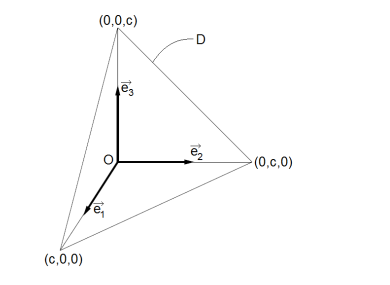
\includegraphics[width=0.45\textwidth]{images/contraintes.png}
\end{center}
\end{boiteexercice}

\begin{boitecorrige}
Le tenseur de Cauchy est symétrique : il y a 6 inconnues $\sigma_{11},\sigma_{22},\sigma_{33},\sigma_{12},\sigma_{13},\sigma_{23}$.

\textbf{Termes diagonaux.} Sur la face de normale sortante $-\vec{e}_1$, le vecteur contrainte est $\vec{T}(-\vec{e}_1)=-\overline{\overline{\sigma}}\cdot\vec{e}_1 = (-\sigma_{11},-\sigma_{12},-\sigma_{13})^T$. La composante normale (projection sur $-\vec{e}_1$) vaut $\sigma_{11}$. La surface de cette facette triangulaire est $S = c^2/2$, donc :
\[
F_1 = S\,\sigma_{11} \Longrightarrow \sigma_{11} = \frac{2F_1}{c^2}
\]
Par des raisonnements identiques sur les deux autres facettes :
\[
\sigma_{22} = \frac{2F_2}{c^2}, \qquad \sigma_{33} = \frac{2F_3}{c^2}
\]

\textbf{Termes hors-diagonaux.} La face inclinée a pour normale unitaire sortante $\vec{n} = \frac{1}{\sqrt{3}}(\vec{e}_1+\vec{e}_2+\vec{e}_3)$ et pour surface $S' = c^2\sqrt{3}/2$. Le vecteur contrainte est :
\[
\vec{T}(\vec{n}) = \frac{1}{\sqrt{3}}\begin{pmatrix}\sigma_{11}+\sigma_{12}+\sigma_{13}\\\sigma_{12}+\sigma_{22}+\sigma_{23}\\\sigma_{13}+\sigma_{23}+\sigma_{33}\end{pmatrix}
\]
La force sur cette facette vaut $\vec{G} = S'\,\vec{T}(\vec{n})$.

En substituant les termes diagonaux et en résolvant le système :
\[
\begin{cases}
\sigma_{12}+\sigma_{13} = (2G_1-2F_1)/c^2\\[2pt]
\sigma_{12}+\sigma_{23} = (2G_2-2F_2)/c^2\\[2pt]
\sigma_{13}+\sigma_{23} = (2G_3-2F_3)/c^2
\end{cases}
\]
En ajoutant les trois équations et en divisant par 2 :
\[
\sigma_{12}+\sigma_{13}+\sigma_{23} = \frac{(G_1+G_2+G_3)-(F_1+F_2+F_3)}{c^2}.
\]

En soustrayant chaque équation, on obtient finalement :
\begin{align*}
\sigma_{12} &= \frac{(G_1-F_1)+(G_2-F_2)-(G_3-F_3)}{c^2}\\
\sigma_{13} &= \frac{(G_1-F_1)-(G_2-F_2)+(G_3-F_3)}{c^2}\\
\sigma_{23} &= \frac{-(G_1-F_1)+(G_2-F_2)+(G_3-F_3)}{c^2}
\end{align*}
\end{boitecorrige}

\subsection*{Exercice 16 - Cisaillement simple \niveau{\facile}}

\begin{boiteexercice}
Un bloc élastique cubique de côté $a$, soumis à un cisaillement simple dans le plan $(x,y)$, a pour tenseur des contraintes :
\[
\sigma = \begin{pmatrix} 0 & \tau & 0 \\ \tau & 0 & 0 \\ 0 & 0 & 0 \end{pmatrix}.
\]
\begin{enumerate}
  \item Calculer les contraintes principales et les directions principales.
  \item Tracer le cercle de Mohr et déterminer la contrainte tangentielle maximale.
  \item Pour $\tau = 50\;\text{MPa}$, donner les valeurs des contraintes principales.
\end{enumerate}
\end{boiteexercice}

\begin{boitecorrige}

\textbf{1. Contraintes principales.}

Le polynôme caractéristique de $\sigma$ est $\det(\sigma - \lambda I) = -\lambda(\lambda^2 - \tau^2) = 0$, dont les racines sont :
\[
\sigma_1 = \tau, \quad \sigma_2 = -\tau, \quad \sigma_3 = 0.
\]
Les directions principales associées dans le plan $(x,y)$ sont à $\pm 45°$ des axes $x$ et $y$ :
\[
\hat{e}_1 = \frac{1}{\sqrt{2}}(\hat{e}_x + \hat{e}_y), \quad \hat{e}_2 = \frac{1}{\sqrt{2}}(\hat{e}_x - \hat{e}_y).
\]

\textbf{2. Cercle de Mohr.}

Dans le plan $(\sigma, \tau)$, le cercle de Mohr dans le plan de cisaillement a pour centre $(0, 0)$ et rayon $\tau$. Le cercle passe par les points $(\pm\tau, 0)$ (contraintes principales) et $(0, \pm\tau)$ (plans à 45°). La contrainte tangentielle maximale est donc :
\[
\tau_\text{max} = \tau.
\]

\textbf{3. Application numérique.}

Pour $\tau = 50\;\text{MPa}$ :
\[
\sigma_1 = +50\;\text{MPa}, \quad \sigma_2 = -50\;\text{MPa}, \quad \sigma_3 = 0.
\]
C'est un état de \emph{traction pure} dans la direction à $+45°$ et \emph{compression pure} dans la direction à $-45°$. Cette propriété est exploitée pour expliquer pourquoi un matériau fragile en cisaillement casse selon des plans à 45° (failure en traction).

\reponse{$\sigma_{1,2} = \pm\tau$, directions à $\pm 45°$ ; $\tau_\text{max} = \tau$}
\end{boitecorrige}

\subsection*{Exercice 17 - Équation de Navier-Stokes incompressible \niveau{\difficile}}

\begin{boiteexercice}
On considère un écoulement incompressible newtonien de densité $\rho$ et de viscosité dynamique $\mu$, régi par l'équation de Navier-Stokes :
\[
\rho\!\left(\frac{\partial\vec{v}}{\partial t} + (\vec{v}\cdot\grad)\vec{v}\right) = -\grad p + \mu\,\Delta\vec{v} + \rho\vec{f}.
\]
\begin{enumerate}
  \item Énoncer l'équation de continuité pour un écoulement incompressible.
  \item Montrer que pour un écoulement permanent ($\partial_t\vec{v}=0$) et sans forces volumiques ($\vec{f}=0$), la pression se calcule à partir de $\vec{v}$ par une équation de Poisson.
  \item Cas d'application : écoulement de Poiseuille plan entre deux plaques parallèles distantes de $2h$, gradient de pression $-G$. Donner le profil $v_x(y)$ et le débit volumique par unité de largeur.
\end{enumerate}
\end{boiteexercice}

\begin{boitecorrige}

\textbf{1. Continuité.}

La conservation de la masse pour un fluide incompressible ($\rho = $ cste) donne :
\[
\div\vec{v} = 0.
\]

\textbf{2. Équation de Poisson pour la pression.}

Pour un écoulement permanent sans forces volumiques :
\[
\rho(\vec{v}\cdot\grad)\vec{v} = -\grad p + \mu\,\Delta\vec{v}.
\]
En prenant la divergence des deux côtés et utilisant $\div\vec{v} = 0$ :
\[
\div\!\left[(\vec{v}\cdot\grad)\vec{v}\right] = -\Delta p + \mu\,\div(\Delta\vec{v}) = -\Delta p + \mu\,\Delta(\div\vec{v}) = -\Delta p.
\]
Donc :
\[
\Delta p = -\rho\,\div\!\left[(\vec{v}\cdot\grad)\vec{v}\right].
\]
C'est une équation de Poisson pour $p$, dont le second membre est connu dès que $\vec{v}$ est donné. Elle est utilisée dans les méthodes numériques de projection (Chorin) pour imposer l'incompressibilité.

\textbf{3. Écoulement de Poiseuille plan.}

Entre deux plaques en $y=\pm h$, le profil est unidirectionnel $\vec{v} = v_x(y)\hat{e}_x$. L'équation stationnaire devient :
\[
0 = -\frac{\d p}{\d x} + \mu\frac{\d^2 v_x}{\d y^2}.
\]
Avec $\d p/\d x = -G$ (gradient de pression constant) et $v_x(\pm h) = 0$ (non-glissement), on intègre deux fois :
\[
v_x(y) = \frac{G}{2\mu}(h^2 - y^2).
\]
Le profil est parabolique, maximal au centre ($v_\text{max} = Gh^2/(2\mu)$). Le débit volumique par unité de largeur :
\[
Q/L = \int_{-h}^{h} v_x(y)\,\d y = \frac{G}{2\mu}\!\left[h^2\cdot 2h - \frac{2h^3}{3}\right] = \frac{2Gh^3}{3\mu}.
\]
La vitesse moyenne est $\bar{v} = Q/(2hL) = Gh^2/(3\mu) = \tfrac{2}{3}v_\text{max}$.

\reponse{$v_x(y) = \dfrac{G}{2\mu}(h^2-y^2)$, \quad $Q/L = \dfrac{2Gh^3}{3\mu}$}
\end{boitecorrige}

\subsection*{Exercice 18 - Onde longitudinale dans une barre élastique \niveau{\moyen}}

\begin{boiteexercice}
On considère une barre élastique homogène de module d'Young $E$ et de masse volumique $\rho$, occupant l'axe $x\in[0,L]$. On note $u(x,t)$ le déplacement longitudinal.
\begin{enumerate}
  \item Établir l'équation d'onde par un bilan de forces sur un élément $\d x$.
  \item Donner la vitesse de propagation $c$ de l'onde.
  \item Application : barre en acier ($E = 200\;\text{GPa}$, $\rho = 7800\;\text{kg\,m}^{-3}$). Calculer $c$.
\end{enumerate}
\end{boiteexercice}

\begin{boitecorrige}

\textbf{1. Équation d'onde.}

Sur un élément $\d x$ de section $S$, la force à gauche est $F(x) = S\sigma_{xx} = SE\,\partial_x u$ (loi de Hooke 1D). Celle à droite est $F(x+\d x) = F(x) + \partial_x F\,\d x$. La masse est $\rho S\,\d x$. Par Newton :
\[
\rho S\,\d x\,\frac{\partial^2 u}{\partial t^2} = \partial_x F\,\d x = SE\,\frac{\partial^2 u}{\partial x^2}\,\d x.
\]
En simplifiant :
\[
\frac{\partial^2 u}{\partial t^2} = \frac{E}{\rho}\,\frac{\partial^2 u}{\partial x^2}.
\]

\textbf{2. Vitesse de propagation.}

L'équation est de type d'Alembert avec :
\[
c = \sqrt{E/\rho}.
\]

\textbf{3. Application acier.}

\[
c = \sqrt{\frac{200\times 10^9}{7800}} \approx 5064\;\text{m\,s}^{-1}.
\]
C'est la vitesse du son dans l'acier (valeur typique $5000$--$6000\;\text{m\,s}^{-1}$ selon l'alliage). On peut comparer avec la vitesse du son dans l'air ($\sim 340\;\text{m\,s}^{-1}$) : la barre solide transmet les vibrations 15 fois plus vite.

\reponse{$c = \sqrt{E/\rho} \approx 5\;\text{km\,s}^{-1}$ pour l'acier}
\end{boitecorrige}

\subsection*{Exercice 19 - Équilibre d'un barrage poids \niveau{\moyen}}

\begin{boiteexercice}
Un barrage poids triangulaire de hauteur $H$ et de largeur à la base $B$ retient une eau de densité $\rho_e$ sur sa face verticale amont. La masse volumique du béton est $\rho_b$.
\begin{enumerate}
  \item Calculer la résultante des forces de pression de l'eau sur le barrage.
  \item Calculer le moment de renversement par rapport au pied aval.
  \item Condition de non-renversement : $B/H \ge ?$ en fonction de $\rho_b/\rho_e$.
\end{enumerate}
\end{boiteexercice}

\begin{boitecorrige}

\textbf{1. Résultante des forces de pression.}

La pression hydrostatique à profondeur $z$ (depuis la surface libre) vaut $p(z) = \rho_e g z$. Sur la face verticale de hauteur $H$, la force par unité de largeur est :
\[
F = \int_0^H p(z)\,\d z = \rho_e g \frac{H^2}{2}.
\]
Le point d'application est à $2H/3$ de la surface libre, soit $H/3$ au-dessus de la base.

\textbf{2. Moment de renversement.}

Le moment de la force $F$ par rapport au pied aval (situé à la base, côté eau) vaut :
\[
M_\text{renv} = F \times \frac{H}{3} = \frac{\rho_e g H^3}{6}.
\]

\textbf{3. Condition de stabilité.}

Le poids du barrage par unité de largeur (triangle de hauteur $H$ et base $B$) :
\[
P = \rho_b g \frac{BH}{2}.
\]
Le centre de gravité du triangle est à $B/3$ du pied aval. Le moment stabilisant :
\[
M_\text{stab} = P \times \frac{B}{3} = \rho_b g \frac{BH}{2}\cdot\frac{B}{3} = \frac{\rho_b g B^2 H}{6}.
\]
Condition de non-renversement ($M_\text{stab} \ge M_\text{renv}$) :
\[
\frac{\rho_b g B^2 H}{6} \ge \frac{\rho_e g H^3}{6} \quad\Rightarrow\quad \frac{B^2}{H^2} \ge \frac{\rho_e}{\rho_b} \quad\Rightarrow\quad \frac{B}{H} \ge \sqrt{\frac{\rho_e}{\rho_b}}.
\]
Pour $\rho_b/\rho_e \approx 2{,}4$ (béton/eau), on obtient $B/H \ge 1/\sqrt{2{,}4} \approx 0{,}65$. En pratique, on prend $B/H \ge 0{,}7$ à $0{,}8$ pour inclure un coefficient de sécurité.

\reponse{$\dfrac{B}{H} \ge \sqrt{\dfrac{\rho_e}{\rho_b}} \approx 0{,}65$ pour béton/eau}
\end{boitecorrige}

\subsection*{Exercice 20 - Tenseur des déformations et rotationnel \niveau{\difficile}}

\begin{boiteexercice}
Soit le champ de déplacement :
\[
\vec{u}(x,y,z) = (\alpha xy,\, \beta xz,\, \gamma yz)
\]
où $\alpha, \beta, \gamma$ sont des constantes petites.
\begin{enumerate}
  \item Calculer la matrice jacobienne $\grad\vec{u}$.
  \item En déduire le tenseur des petites déformations $\epsilon$ et le tenseur rotationnel $\omega$.
  \item Vérifier la compatibilité géométrique (équations de Saint-Venant).
\end{enumerate}
\end{boiteexercice}

\begin{boitecorrige}

\textbf{1. Jacobienne.}

\[
\grad\vec{u} = \begin{pmatrix}
\partial_x u_x & \partial_y u_x & \partial_z u_x \\
\partial_x u_y & \partial_y u_y & \partial_z u_y \\
\partial_x u_z & \partial_y u_z & \partial_z u_z
\end{pmatrix} = \begin{pmatrix}
\alpha y & \alpha x & 0 \\
0 & 0 & \beta x \\
0 & \gamma z & \gamma y
\end{pmatrix}.
\]

\textbf{2. Déformations et rotation.}

Le tenseur des déformations (partie symétrique) :
\[
\epsilon = \frac{1}{2}(\grad\vec{u} + {}^t\!\grad\vec{u}) = \begin{pmatrix}
\alpha y & \alpha x/2 & 0 \\
\alpha x/2 & 0 & \beta x/2 + \gamma z/2 \\
0 & \beta x/2 + \gamma z/2 & \gamma y
\end{pmatrix}.
\]
Le tenseur rotation (partie antisymétrique) :
\[
\omega = \frac{1}{2}(\grad\vec{u} - {}^t\!\grad\vec{u}) = \begin{pmatrix}
0 & \alpha x/2 & 0 \\
-\alpha x/2 & 0 & \beta x/2 - \gamma z/2 \\
0 & -\beta x/2 + \gamma z/2 & 0
\end{pmatrix}.
\]
Le vecteur rotation associé est $\vec{\Omega} = \tfrac{1}{2}\rot\vec{u} = \tfrac{1}{2}\bigl(\partial_y u_z - \partial_z u_y,\, \partial_z u_x - \partial_x u_z,\, \partial_x u_y - \partial_y u_x\bigr) = \tfrac{1}{2}(\gamma z,\, 0,\, -\alpha x)$.

\textbf{3. Compatibilité de Saint-Venant.}

Les équations de compatibilité assurent que les $\epsilon_{ij}$ proviennent bien d'un champ de déplacement unique. Elles s'écrivent :
\[
\partial_{kl}\epsilon_{ij} + \partial_{ij}\epsilon_{kl} = \partial_{ik}\epsilon_{jl} + \partial_{jl}\epsilon_{ik}.
\]
Pour le champ donné, par exemple $\partial_y\epsilon_{xx} = \alpha$, $\partial_{xy}\epsilon_{xy} = \alpha/2$. Vérifions une équation :
\[
\partial_{yy}\epsilon_{xx} + \partial_{xx}\epsilon_{yy} = 0 + 0 = 0, \qquad 2\partial_{xy}\epsilon_{xy} = 2\times\frac{\alpha}{2} = \alpha.
\]
Pour compatibilité : $0 = \alpha$, soit $\alpha = 0$. Cela signifie que le champ $\vec{u}$ n'est physiquement compatible que si $\alpha = 0$. Plus généralement, les équations de Saint-Venant imposent ici $\alpha = \beta = \gamma = 0$ : le champ n'est pas physiquement réalisable en petites déformations. C'est un exemple pédagogique de l'importance des conditions de compatibilité.

\reponse{$\epsilon_{ij} = \tfrac{1}{2}(\partial_i u_j + \partial_j u_i)$ ; champ non compatible sauf si $\alpha=\beta=\gamma=0$}
\end{boitecorrige}

\ifdefined\inMainDoc\else\end{document}\fi
